\section{Data and Study Design}
\label{sec:data-design}

\begin{figure*}[t]
  \centering
  \begin{tikzpicture}[
    node distance=6mm and 9mm,
    box/.style={draw=cvprblue!80!black, fill=cvprblue!8, rounded corners=2pt, align=center,
                font=\scriptsize, minimum height=11mm, text width=4.6cm, inner sep=3pt},
    post/.style={box, fill=orange!10, draw=orange!70!black},
    arr/.style={-{Stealth[length=2mm]}, thick, draw=black!70}]
    % row 1 (left to right)
    \node[box] (n1) {\textbf{1. Decision frame}\\support officer $\cdot$ after semester 1\\Dropout vs.\ Graduate $\cdot$ top-20\% capacity};
    \node[box, right=of n1] (n2) {\textbf{2. Data design}\\UCI 4,424 $\rightarrow$ 3,630 records $\cdot$ no 2nd-semester data\\frozen 70/15/15 split IDs (seed 42)};
    \node[box, right=of n2] (n3) {\textbf{3. Model development}\\train-only preparation\\\tabicl + LR / tree / XGBoost / EBM};
    % row 2 (right to left)
    \node[box, below=of n3] (n4) {\textbf{4. Validation freeze}\\model $\cdot$ top-20\% outreach rule\\SHAP groups and budget $\cdot$ hashed snapshot};
    \node[box, below=of n2] (n5) {\textbf{5. One-time final test} (2 Nov)\\performance $\cdot$ calibration $\cdot$ subgroups\\paired bootstrap $\cdot$ lock file};
    \node[box, below=of n1] (n6) {\textbf{6. Local explanations}\\permutation SHAP $\cdot$ semantic groups\\study cases exported};
    % row 3 (left to right)
    \node[post, below=of n6] (n7) {\textbf{7. Explanation evidence} (post-hoc)\\544 validation students: deletion $\cdot$ stability\\recourse $\cdot$ surrogates $\cdot$ sensitivity checks};
    \node[box, below=of n5] (n8) {\textbf{8. Human study}\\50 participants, two groups, Google Forms\\forward simulation $\cdot$ qualitative coding};
    \node[post, below=of n4] (n9) {\textbf{9. Deliverables}\\report $\cdot$ code $\cdot$ aggregate tables $\cdot$ model card\\local research interface};
    \draw[arr] (n1) -- (n2); \draw[arr] (n2) -- (n3); \draw[arr] (n3) -- (n4);
    \draw[arr] (n4) -- (n5); \draw[arr] (n5) -- (n6); \draw[arr] (n6) -- (n7);
    \draw[arr] (n7) -- (n8); \draw[arr] (n8) -- (n9);
  \end{tikzpicture}
  \caption{Research workflow as carried out (updated from the proposal). The model, outreach rule and
  explanation settings were frozen on validation data before the one-time final test. Orange steps (the
  full explanation audit, the validation-only sensitivity checks and the local interface) were
  completed after the final test without changing the model. Ethics, governance and reproducibility
  apply throughout.}
  \label{fig:project-pipeline}
\end{figure*}


\subsection{Dataset and Target}

The study uses the UCI \emph{Predict Students' Dropout and Academic Success} dataset (repository
dataset 697, CC~BY~4.0)~\citep{realinho2021uci, realinho2022predicting}, which describes 4,424
students from a Portuguese higher-education institution with 36 predictors and three outcomes:
Dropout (1,421), Enrolled (794) and Graduate (2,209). The distributed file contains no direct
identifiers, missing values or duplicate rows. The task is binary, Dropout (1) versus Graduate (0),
yielding 3,630 records. Enrolled students were excluded since their final outcome is unknown. This
exclusion is a genuine limitation: at the moment of decision every student is enrolled, so a
deployed model would also score students resembling those removed. Section~\ref{sec:sensitivity}
examines how the model treats them.

\textbf{Eligibility.} Of the dropouts, 17.3\% (246 of 1,421) took no first-semester evaluations,
compared with only 3.4\% of graduates (75 of 2,209). Some labelled dropouts may therefore have left
before the decision point rather than after it, in which case not every flagged ``dropout'' could
still have been reached by a support meeting. This timing ambiguity is reported as an explicit
eligibility limitation; Section~\ref{sec:who} analyses who is flagged, and
Section~\ref{sec:sensitivity} re-ranks students after setting these cases aside.

\textbf{Exploratory data analysis.} Table~\ref{tab:eda} compares dropouts and graduates on the
training split only (2,541 students), leaving the test split uninspected. The classes are moderately
imbalanced (39\% dropout). First-semester results separate the groups most clearly: dropouts passed
2.6 units on average against 6.3 for graduates, and 40\% passed none. Financial indicators also
differ (fees up to date 69\% vs.\ 99\%; debtor 22\% vs.\ 5\%), as do age and gender. These patterns
anticipate both the model's reliance on first-semester progress and the subgroup gaps reported in
Section~\ref{sec:fairness}.

\begin{table}[!htb]
\centering
\caption{Training-split profile by outcome (2,541 students). Average grade is on the 0--20 scale and
is 0 when no unit was passed.}
\label{tab:eda}
\footnotesize
\setlength{\tabcolsep}{4pt}
\begin{tabular}{@{}lcc@{}}
\toprule
\textbf{Characteristic} & \textbf{Dropout} & \textbf{Graduate} \\
\midrule
Students & 995 & 1,546 \\
First-semester units passed (mean) & 2.6 & 6.3 \\
Passed no first-semester unit & 39.6\% & 3.2\% \\
Took no first-semester evaluation & 17.6\% & 3.0\% \\
First-semester average grade (mean) & 7.3 & 12.7 \\
Tuition fees up to date & 68.7\% & 98.6\% \\
Debtor & 21.5\% & 5.0\% \\
Scholarship holder & 9.8\% & 39.1\% \\
Age at enrolment (median) & 23 & 19 \\
Female (gender 0) & 52.4\% & 77.0\% \\
\bottomrule
\end{tabular}
\end{table}

\subsection{Prediction Time and Feature Windows}

The primary feature window is \emph{after the first semester}. It contains 30 original attributes
covering background (age, gender, nationality, marital status, displacement and special needs),
application (route, order, course, attendance, prior qualification and grades), family (parents'
education and occupation), finances (scholarship, tuition fees up to date and debtor status),
first-semester units (credited, enrolled, evaluated, passed, without evaluation and average grade)
and national economic indicators. Three derived features complete the 33 inputs: the
first-semester pass rate and indicators for no units enrolled and no evaluations taken. All six
second-semester attributes are removed to prevent leakage of future information, and an
admission-time window without first-semester results serves as a sensitivity analysis.

\subsection{Frozen Split and Outreach Policy}

The 3,630 records were split once, with stratification, into 70/15/15\% train, validation and test
sets (2,541, 544 and 545 records; seed 42), and the row identifiers were saved. Every modelling and
explanation setting was chosen on the validation split. The test split was subsequently used
exactly once, in a run protected by a lock file and a hash of the frozen code, data and model.

The outreach policy flags the $k=\lfloor 0.2n\rfloor$ highest-scoring students in a cohort of size
$n$ (108 of 544 in validation and 109 of 545 in test), breaking ties by record order. Consequently,
there is no universal probability threshold: a student's flag depends on their rank within the
cohort.

\subsection{Human-Study Design and Ethics}

The study applies forward simulation~\citep{hase2020forward}, asking whether people can predict
the model's hidden flag from a student profile. Fifty adult volunteers (a convenience sample, with
about ten recruited by each team member) were assigned by a sealed, seeded list to Group~A (profile
only, $n=25$) or Group~B (profile plus a bar chart of the five largest grouped SHAP contributions,
$n=25$). The chart displayed direction and relative size only, never the score, the base value or
the flag (Figure~\ref{fig:human-design}).

Each participant first completed one unscored practice case from the validation split and then ten
scored test cases (five flagged and five not flagged by the model) in one of two fixed orders, a
seeded order or its exact reverse, yielding four Google Forms. For each case, participants
predicted whether the model had flagged the student, rated their confidence from 1 to 5 and answered
three short written questions: why the model decided as it did, what support they would suggest and
what further information they would want. Group~B additionally answered two chart-reading checks on
the practice case, and all participants self-reported their total completion time.

\textbf{Ethics and data governance.} As a class project, the study followed basic research-ethics
practice (voluntary informed consent, minimal data, no identifiers and restricted access) rather
than formal ethics-board review. All participants were adults, and taking
part or declining had no effect on grades, employment or access to services. No names or AIT
student records were collected; responses carry random participant codes, the case lookup is
stored separately, raw free text is held outside version control with access limited to the team,
and only aggregate results are reported. Participants could withdraw through their code until their
responses entered the aggregate analysis; all 50 completed the study and none were excluded. Raw
responses and case-linkage files remain in access-restricted storage, excluded from the public
repository and used only for this course project, and the written answers
were never used to train, validate or explain the model. The online, unsupervised format is
discussed as a limitation.

\begin{figure}[t]
  \centering
  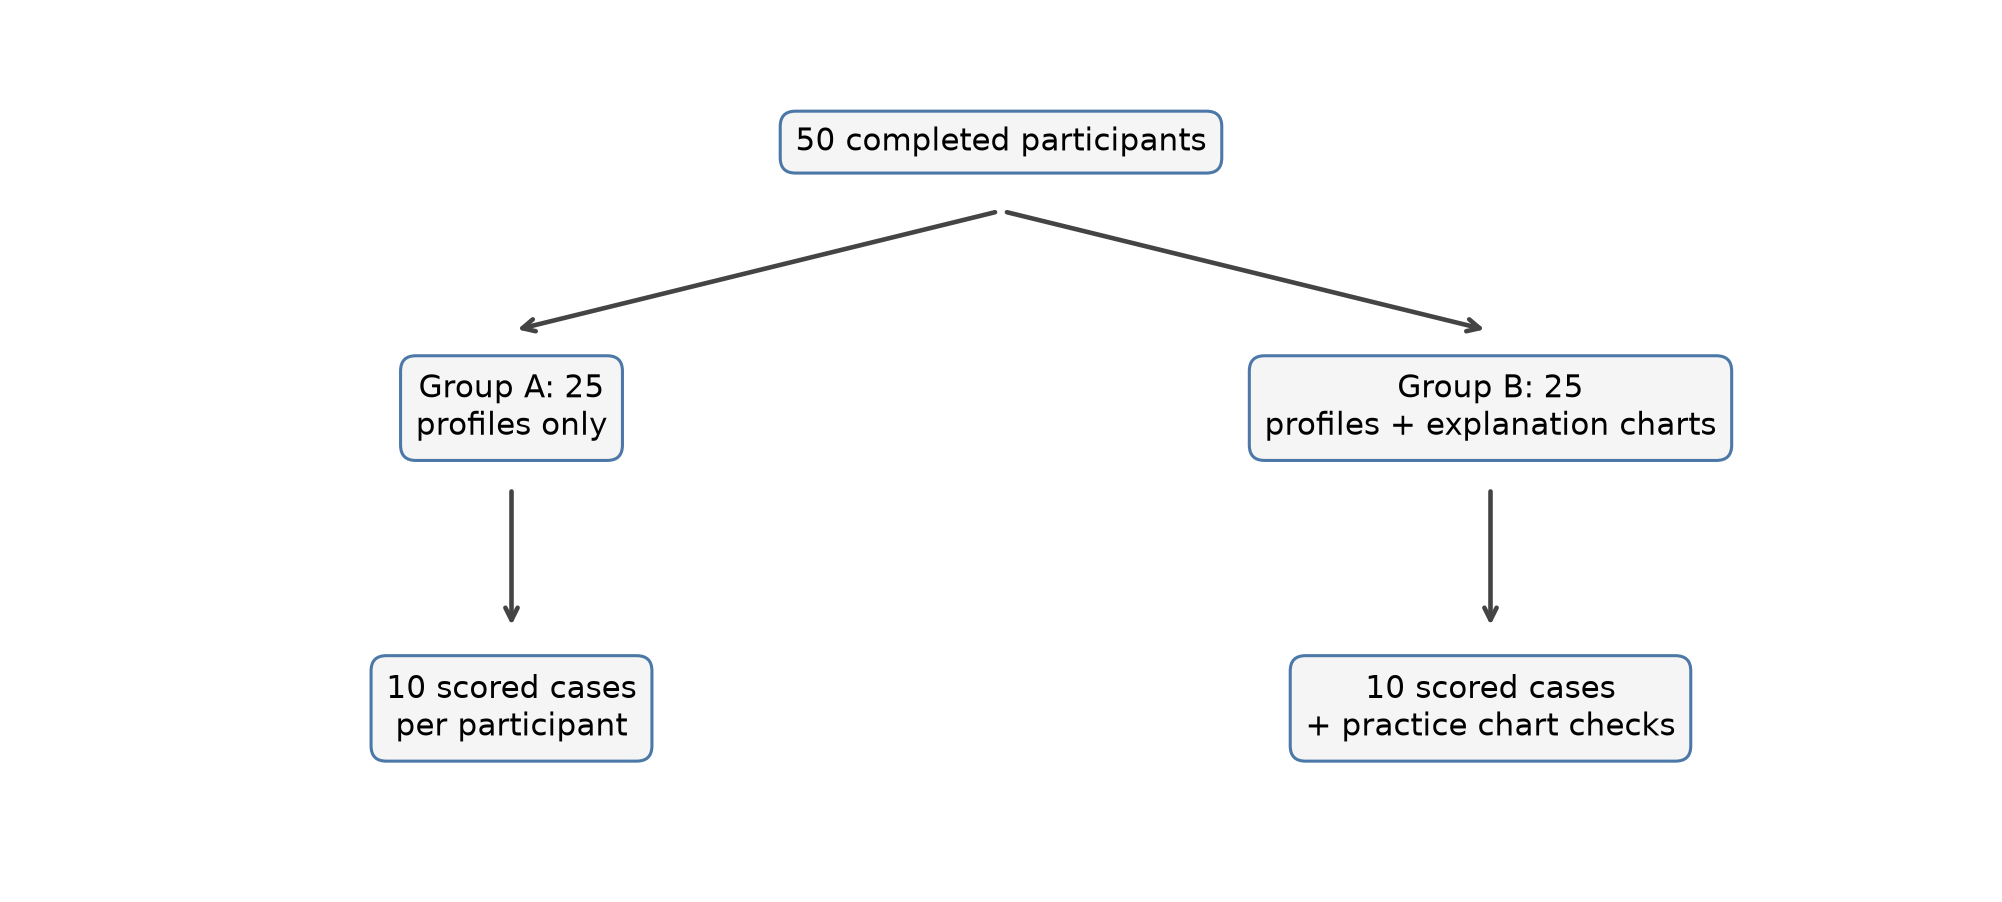
\includegraphics[width=\linewidth]{human_study_design.png}
  \caption{Two-group forward-simulation design: 25 participants per group, one practice case and
  ten scored test cases in two counterbalanced orders.}
  \label{fig:human-design}
\end{figure}
